\section{Building and running}
\label{app:usage}

The only prerequisite is a JDK, version 21 or newer.

\begin{lstlisting}[style=text]
./mvnw package                                    build target/cellula.jar and run the tests
java -jar target/cellula.jar --dir examples       open the menu on the example files
java -jar target/cellula.jar help                 list the commands
\end{lstlisting}

Without arguments, the program lists the definition files of the current directory, as the
subject requires. In the simulation window, the space bar plays or pauses, the right arrow
advances by one generation, and \code{R} goes back to generation 0.

\begin{lstlisting}[style=text]
java -jar target/cellula.jar print examples/sierpinski.xml --steps 31
java -jar target/cellula.jar render examples/crystal-3d.xml --steps 30 --output crystal.png
java -jar target/cellula.jar validate examples/*.xml
java -jar target/cellula.jar explore --family symmetric --samples 50000 --write found
\end{lstlisting}

\section{Reference of the rule language}
\label{app:language}

\begin{lstlisting}[style=text]
rule         := expression
expression   := NUMBER | NAME '(' arguments ')'
arguments    := neighborhood | [ expression { ',' expression } ]
neighborhood := NAME
NUMBER       := '-'? DIGIT+
NAME         := LETTER ( LETTER | DIGIT | '_' )* '*'?
\end{lstlisting}

\begin{table}[H]
    \centering\small
    \begin{tabularx}{\textwidth}{@{}l L l@{}}
        \toprule
        Operator                                             & Value                                                               & Alias        \\
        \midrule
        \code{ET(a, b)}                                      & 1 if \code{a} and \code{b} are both different from 0, else 0        & \code{AND}   \\
        \code{OU(a, b)}                                      & 0 if \code{a} and \code{b} are both equal to 0, else 1              & \code{OR}    \\
        \code{NON(a)}                                        & 1 if \code{a} equals 0, else 0                                      & \code{NOT}   \\
        \code{SUP(a, b)}                                     & 1 if \code{a} is strictly greater than \code{b}, else 0             & \code{GT}    \\
        \code{SUPEQ(a, b)}                                   & 1 if \code{a} is greater than or equal to \code{b}, else 0          & \code{GE}    \\
        \code{EQ(a, b)}                                      & 1 if \code{a} equals \code{b}, else 0                               &              \\
        \code{COMPTER(G)}                                    & number of cells in state 1 in the neighborhood \code{G} of the cell &
        \code{COUNT}                                                                                                                              \\
        \code{ADD(a, b)}, \code{SUB(a, b)}, \code{MUL(a, b)} & sum, difference, product                                            &              \\
        \code{SI(c, a, b)}                                   & \code{a} if \code{c} is different from 0, else \code{b}             & \code{IF}    \\
        \code{ETAT()}                                        & state of the cell itself (extension)                                & \code{STATE} \\
        \bottomrule
    \end{tabularx}
    \caption{The operators of the rule language.}
\end{table}

\section{The example files}
\label{app:examples}

\begin{table}[H]
    \centering\small
    \begin{tabularx}{\textwidth}{@{}l l L@{}}
        \toprule
        File                                                   & Grid           & Demonstrates                                            \\
        \midrule
        \code{game-of-life.xml}                                & $64 \times 96$ & Required: Game of Life from \code{RANDOM(15)}           \\
        \code{sierpinski.xml}                                  & 257            & Required: Sierpi\'nski triangle, formula of the subject \\
        \code{growth.xml}                                      & 41             & Figures 1 and 2 of the subject                          \\
        \code{subject-example.xml}                             & $64 \times 96$ & The rule of section 2.3, verbatim                       \\
        \code{glider.xml}                                      & $20 \times 20$ & Explicit cells, periodic boundary, cycle detection      \\
        \code{rule-30.xml}, \code{rule-110.xml}                & 257            & User-defined one-cell neighborhoods                     \\
        \code{brians-brain.xml}                                & $64 \times 96$ & Three states, colors, \code{ETAT()}                     \\
        \code{snowflake.xml}                                   & $97 \times 97$ & Hexagonal lattice by a user-defined neighborhood        \\
        \code{crystal-3d.xml}                                  & $65^3$         & Three dimensions, G6*, slice \code{(32, :, :)}          \\
        \code{clouds-3d.xml}                                   & $40^3$         & Three dimensions, G26*, random start                    \\
        \code{hypercube-4d.xml}                                & $25^4$         & Four dimensions, slice \code{(:, :, 12, 12)}            \\
        \code{radius2-fractal.xml}, \code{radius2-chaotic.xml} & 1\,021         & Bonus question                                          \\
        \bottomrule
    \end{tabularx}
    \caption{The definition files shipped with the project.}
\end{table}

\begin{figure}[H]
    \centering
    \begin{subfigure}[b]{0.31\textwidth}
        \centering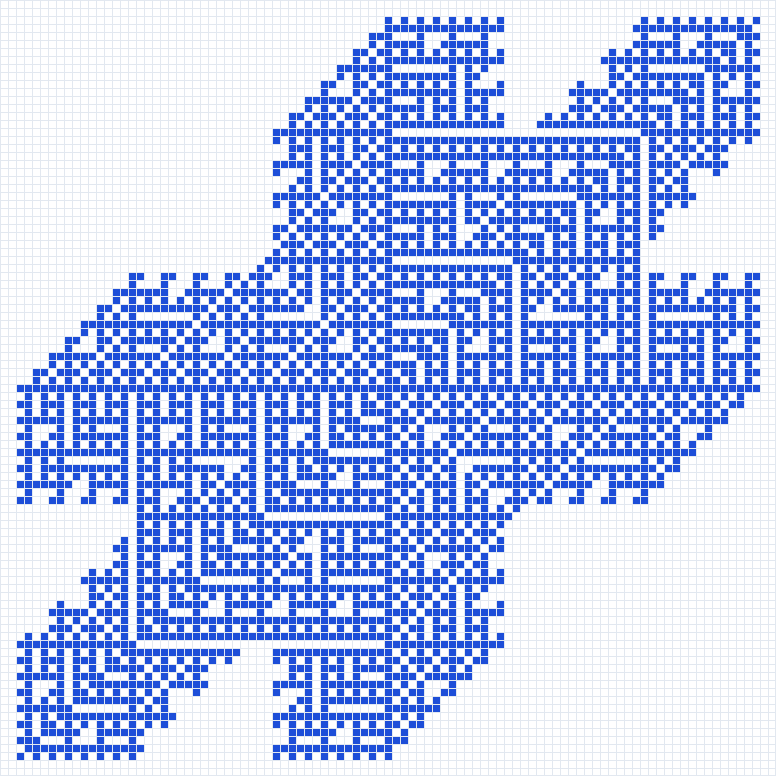
\includegraphics[width=\textwidth]{snowflake}
        \caption{\code{snowflake.xml}}
    \end{subfigure}\hfill
    \begin{subfigure}[b]{0.31\textwidth}
        \centering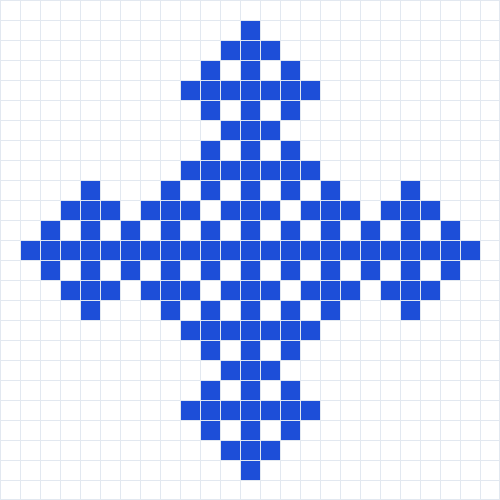
\includegraphics[width=\textwidth]{hypercube-4d}
        \caption{\code{hypercube-4d.xml}}
    \end{subfigure}\hfill
    \begin{subfigure}[b]{0.31\textwidth}
        \centering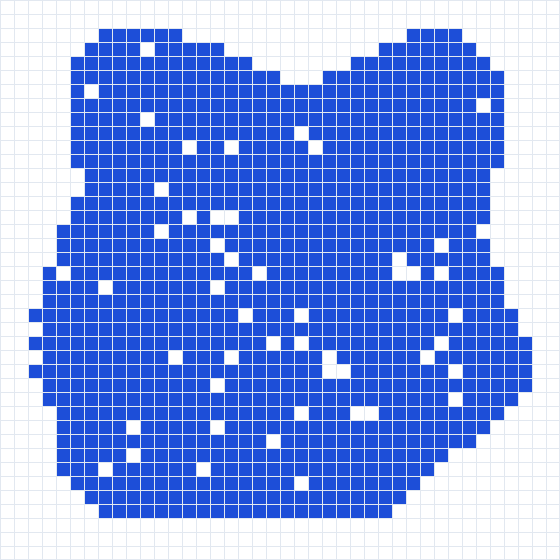
\includegraphics[width=\textwidth]{clouds-3d}
        \caption{\code{clouds-3d.xml}}
    \end{subfigure}\\[0.8em]
    \begin{subfigure}[b]{0.48\textwidth}
        \centering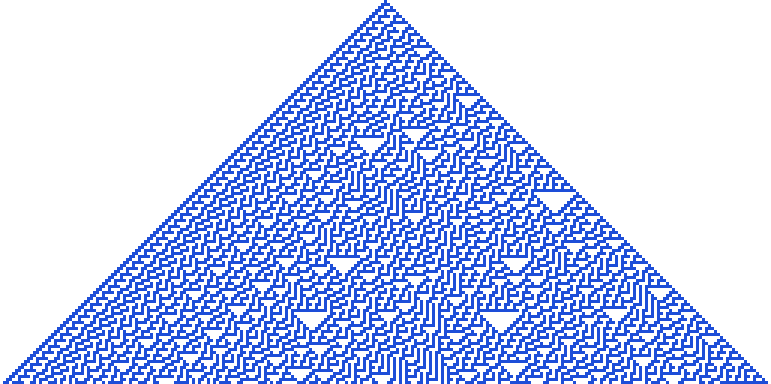
\includegraphics[width=\textwidth]{rule-30}
        \caption{\code{rule-30.xml}}
    \end{subfigure}\hfill
    \begin{subfigure}[b]{0.48\textwidth}
        \centering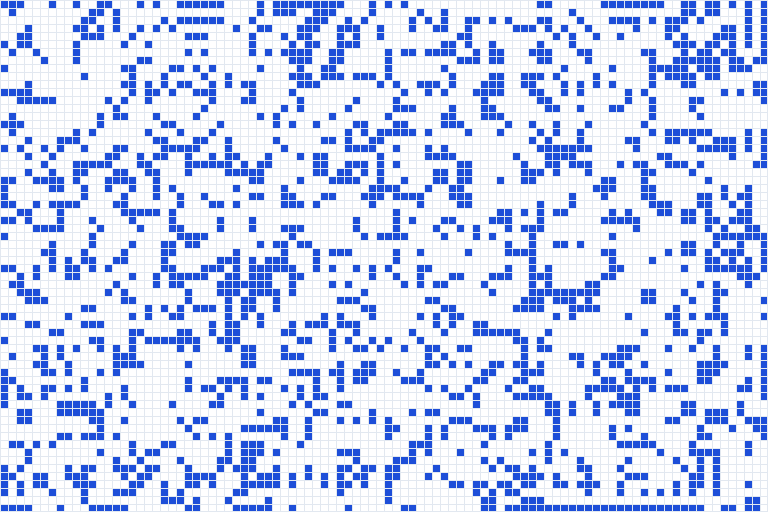
\includegraphics[width=\textwidth]{subject-example}
        \caption{\code{subject-example.xml}}
    \end{subfigure}
    \caption{A few of the examples, rendered by \code{cellula render}.}
\end{figure}
